\subsubsection{Detektion}
\label{subsec:03detektion}
Als grundlegender Schritt der Personenverfolgung muss eine Person in dem Kamerabild gefunden werden. Dieser Vorgang nennt sich (Personen-)Detektion. Herk�mmliche Histogram-of-Oriented-Gradients Ans�tze liefern keine zufriedenstellende L�sung bez�glich des Fahrzeugs. Daher f�llt die Wahl auf die Nutzung eines Convolutional-Neural-Networks kurz CNN. Diese Netze eignen sich sehr gut zur Klassifizierung von Objekten in Bildern, da sie die Zugeh�rigkeit eines Objektes zu einer Klasse mit Wahrscheinlichkeiten ausdr�cken.

Ein typisches CNN besteht aus drei Layern. Das erste ist das Convolutional Layer. Durch die Faltung des Kamerabildes mit einem Kernel bzw. einer Faltungsmatrix werden die Werte der Eingangsschicht berechnet. Die Werte des Kernels sind dabei auf das jeweilige Problem angepasst. Das Ergebnis davon ist eine sogenannte Feature-Map. Werden nun die Ergebnisse der Faltung mit einer Aktivierungsfunktion verkn�pft, bildet dies den Ausgang der einzelnen Neuronen des ersten Layers. Bei CNNs ist die Nutzung einer Rectified Linear Unit (ReLU) definiert durch $f(x) = max(0,x)$ mit $x$ als Ergebnis der Faltung �blich. Die zweite Schicht bildet das Pooling Layer. Hier findet eine Ordnungsreduktion statt, indem �berfl�ssige Informationen verworfen werden. Das geschieht beispielsweise mit einem Max-Pooling. Dabei wandert ein $2 \times 2$-Filter �ber den Ausgang der Neuronen des Convolutional Layers und beh�lt nur die Aktivit�t des jeweils aktivsten Neurons. Der Vorteil dieses Layers ist unter anderem eine erh�hte Berechnungsgeschwindigkeit des gesamten Netzes. Den Abschluss bildet das Fully-connected Layer. Hier werden die Eing�nge des Layers Objektklassen zugeteilt.

Als Neuronales Netz zur Bew�ltigung der urspr�nglichen Aufgabe wird das \textit{Google MobileNet SSD}\cite{mobilenet} als Caffe Framework Modell verwendet, welches bereits vortrainiert ist. Ein weiterer Vorteil dieses Netzes ist die Optimierung auf ressourcenschonende Berechnungen, allerdings auf Kosten der Genauigkeit. Dieser einhergehende Nachteil wird im vorliegenden Anwendungsfall jedoch nicht als relevant erkannt. Diese Optimierung zieht eine �nderung der gew�hnlichen Struktur eines CNNs mit sich wie in Abbildung \ref{fig:pv-neural-net} dargestellt.
\begin{figure}[btp]
	\centering
	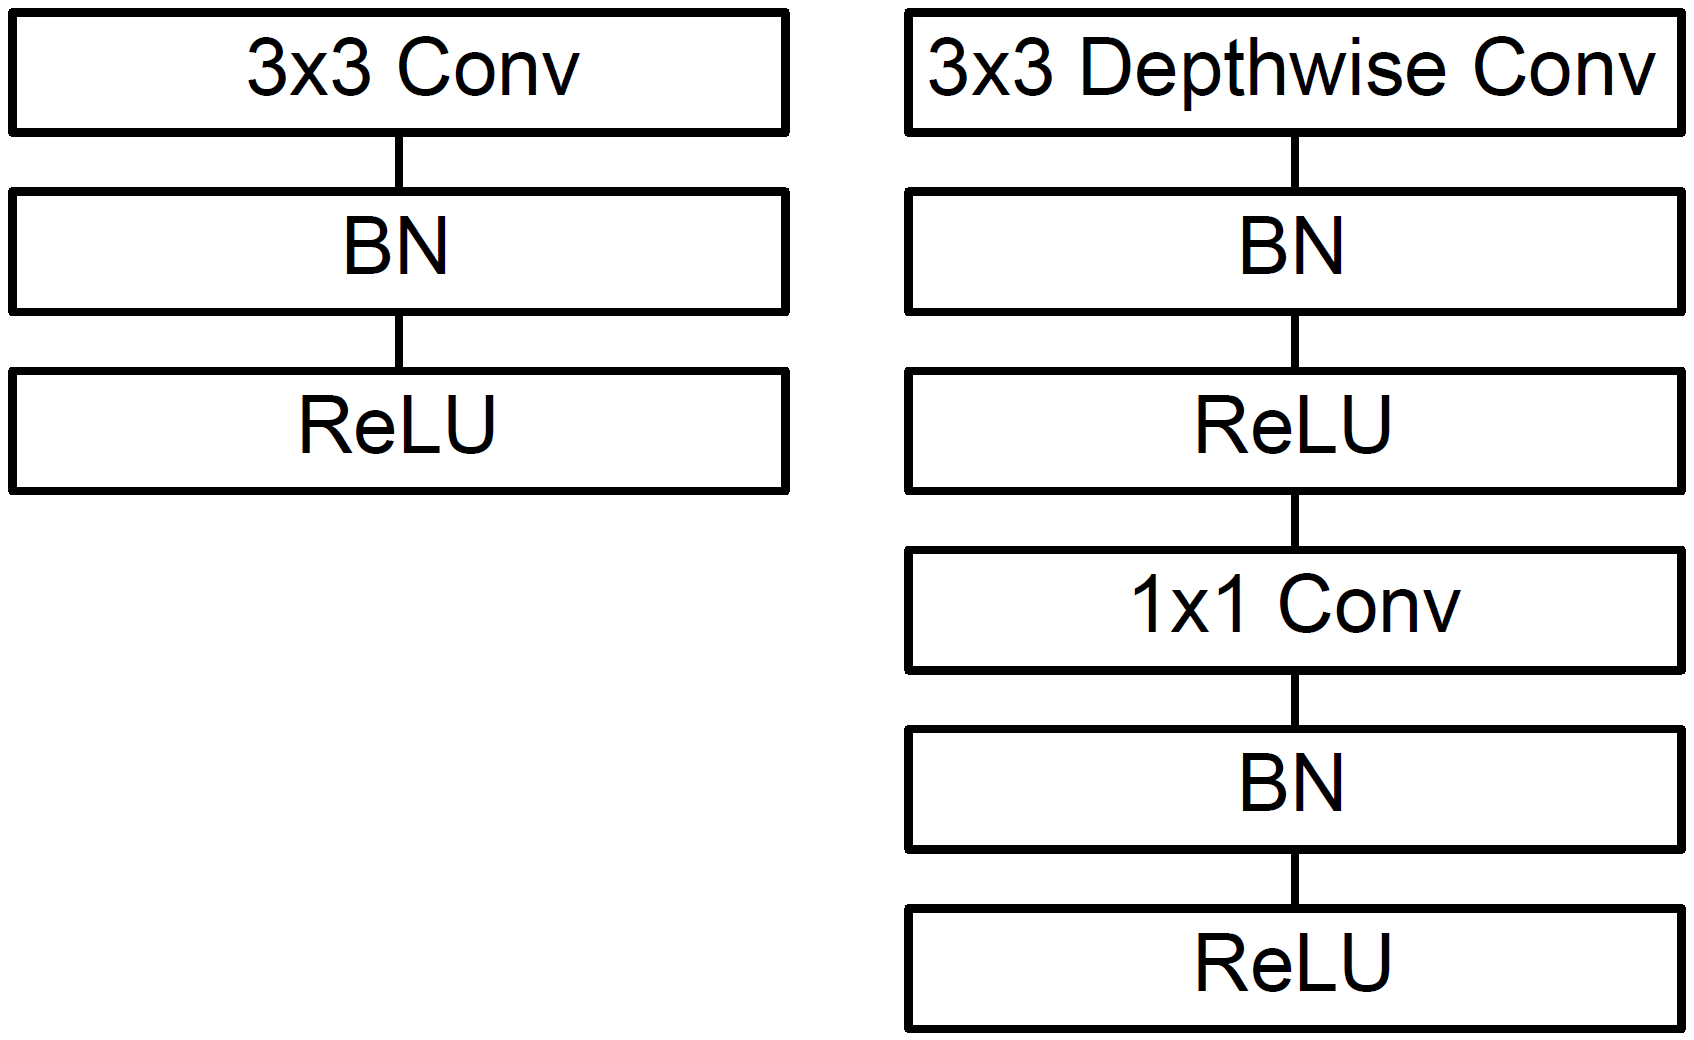
\includegraphics[width=.6\textwidth]{./pics/pv-neural-net.png}
	\caption{Links: Standard Convolutional Layer mit Batch Normalization und ReLU. Rechts: Depthwise Separable Convolutions mit Depthwise und Pointwise Layers gefolgt von Batch Normalization und ReLU. (aus \cite{mobilenet})}
	\label{fig:pv-neural-net}
\end{figure}
Die grundlegende Idee hinter Depthwise Separable Convolution ist die Aufteilung der Faltung eines CNNs in eine $3 \times 3$ Depthwise Convolution gefolgt von einer $1 \times 1$ Pointwise Convolution. Dabei dient Ersteres dazu, jeden Eingangkanal zu filtern und Letzteres dazu, diese Ausg�nge wieder zusammenzuf�hren. Der Vorteil davon ist die drastische Reduzierung des Berechnungsaufwands und der Modellgr��e. Batch Normalization\footnote{https://towardsdatascience.com/batch-normalization-in-neural-networks-1ac91516821c} bezeichnet dabei die Normalisierung der Werte der unsichtbaren Schichten des Netzes, um die Trainingsgeschwindigkeit deutlich zu erh�hen.

Benutzt wird das Netz mithilfe des seit OpenCV 3.3 existierenden Deep Neural Networks (dnn) Moduls. Dieses kann unter anderem Caffe Framework Modelle laden, benutzen und trainieren. Letztere Funktion wird nicht benutzt, da das Netz bereits ausreichend trainiert ist. Daher muss es lediglich einmalig zum Programmstart geladen werden. Der aktuelle Kameraframe des Farbbildes wird auf eine Gr��e von \SI{300}{px}$\times$\SI{300}{px} skaliert, da das Netz ein Eingangsbild dieser Gr��e erwartet. Anschlie�end wird der Frame vorverarbeitet. Einerseits erfolgt mit einer sogenannten Mean Subtraction eine Subtraktion des Durchschnitts des jeweiligen Farbkanals vom Kameraframe, um Helligkeitsunterschieden entgegen zu wirken. Dabei wird hier der Durchschnitt auf allen Farbkan�len zu $\mu = 127,5$ gew�hlt. Andererseits kann diese Subtraktion mithilfe eines Skalierungsparameters $\sigma$ normalisiert werden. Hier wird $\sigma = 127,502231$ gew�hlt. Zu beachten ist, dass der an die \textit{blobFromImage}-Funktion �bergebende Skalierungsfaktor $1/\sigma$ entspricht. Anschlie�end kann der eben erstellte Blob dem Netz als Eingang �bergeben werden. Die Ausgabe beinhaltet alle erkannten Objekte als Matrix zusammengefasst. Eine Zeile dieser Matrix besteht aus den Eintr�gen $d^T = [0, \text{ID der zugeh�rigen Klasse}, \text{Wahrscheinlichkeit}, x, y, \text{Breite}, \text{H�he}]$. Dabei liegen die Werte der $x$- und $y$-Koordinate im Bereich $[0, 1]$ und m�ssen, um die eigentlichen Koordinaten zu erhalten, erst mit der Bildbreite bzw. Bildh�he multipliziert werden. Da unter Umst�nden mehrere Personen im Bild detektiert werden k�nnen, wird diejenige ausgew�hlt, die die gr��te Klassenwahrscheinlichkeit besitzt. Eine Alternative w�re, zus�tzlich die Wahl der Personen auf einen Bereich um den Bildmittelpunkt zu begrenzen, wenn davon ausgegangen wird, dass die zu detektierende Person frontal vor dem Fahrzeug steht. Nun ist die gew�nschte Person detektiert und es kann mithilfe der angesprochenen Koordinatentransformation eine Bounding-Box der Person f�r die nachfolgenden Module erstellt werden.